
\section{Introduction to Mixed Number}

In this lesson, we will learn the definition of mixed numbers, and how to convert between improper fraction (like $\frac{3}{2}$) and mixed number (like $1 \frac{1}{2}$).

\subsection{Definition of Mixed Number}

Let's review the definition of fractions, and use $\frac{2}{3}$ as an example. Remember, we should look at the denominator, $3$, first:
\begin{enumerate}
\item We cut the whole evenly into $3$ pieces.
\item We take $2$ of those pieces.
\end{enumerate}

\begin{center}
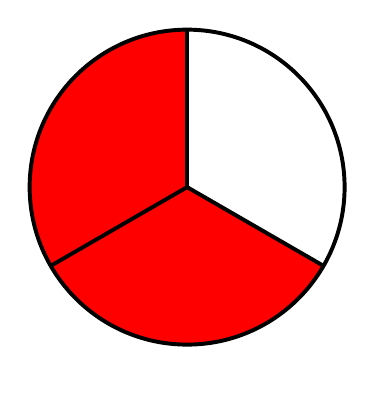
\begin{tikzpicture}
	\fill[red] (0,0) -- (0,2) arc (90:210:2cm) -- cycle;
	\fill[red] (0,0) -- (-2*0.8661,-2*0.5) arc (210:330:2cm) -- cycle;
	\draw[line width=0.5mm] (0,0) circle (2cm);
	\draw[line width=0.5mm] (0,0) -- (0,2);
	\draw[line width=0.5mm] (0,0) -- (2*0.8661,-2*0.5);
	\draw[line width=0.5mm] (0,0) -- (-2*0.8661,-2*0.5);
\end{tikzpicture}
\captionof{figure}{Red pieces in the pie represent $\frac{2}{3}$}
\end{center}

Let's use the same concept to draw $\frac{7}{3}$.
\begin{enumerate}
\item We cut the whole evenly into $3$ pieces.
\item We take $7$ of those pieces. Since one pie only has $3$ pieces, we need to cut more than one pie to have $7$ pieces.
\end{enumerate}

\begin{center}
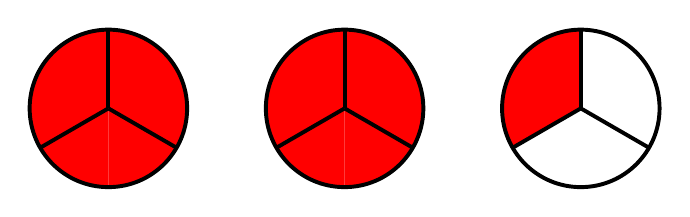
\begin{tikzpicture}
	\fill[red] (0,0) -- (0,1) arc (90:270:1cm) -- cycle;
	\fill[red] (0,0) -- (0,1) arc (90:-90:1cm) -- cycle;
	\draw[line width=0.5mm] (0,0) circle (1cm);
	\draw[line width=0.5mm] (0,0) -- (0,1);
	\draw[line width=0.5mm] (0,0) -- (0.8661,-0.5);
	\draw[line width=0.5mm] (0,0) -- (-0.8661,-0.5);
	
	\fill[red] (3,0) -- (3,1) arc (90:270:1cm) -- cycle;
	\fill[red] (3,0) -- (3,1) arc (90:-90:1cm) -- cycle;
	\draw[line width=0.5mm] (3,0) circle (1cm);
	\draw[line width=0.5mm] (3,0) -- (3,1);
	\draw[line width=0.5mm] (3,0) -- (0.8661+3,-0.5);
	\draw[line width=0.5mm] (3,0) -- (-0.8661+3,-0.5);
	
	\fill[red] (6,0) -- (6,1) arc (90:210:1cm) -- cycle;
	\draw[line width=0.5mm] (6,0) circle (1cm);
	\draw[line width=0.5mm] (6,0) -- (6,1);
	\draw[line width=0.5mm] (6,0) -- (0.8661+6,-0.5);
	\draw[line width=0.5mm] (6,0) -- (-0.8661+6,-0.5);
	
\end{tikzpicture}
\captionof{figure}{Red pieces represent $\frac{7}{3}$}
\end{center}

If the numerator is bigger than the denominator, like in $\frac{7}{3}$, this fraction is called an \textit{improper fraction}.

Another way to write $\frac{7}{3}$ is $2 \frac{1}{3}$, representing $2$ whole pies plus $\frac{1}{3}$ of a pie. A fraction like $2 \frac{1}{3}$ is called a \textit{mixed number}.

In other words, each mixed number can be converted to an improper fraction, and vice versa:
\[ \frac{7}{3} = 2\frac{1}{3} \]

\subsection{Convert between Improper Fractions and Mixed Numbers}
Let's look at one more example by graphing. Write a mixed number and an improper fraction for the following graph:

\begin{center}
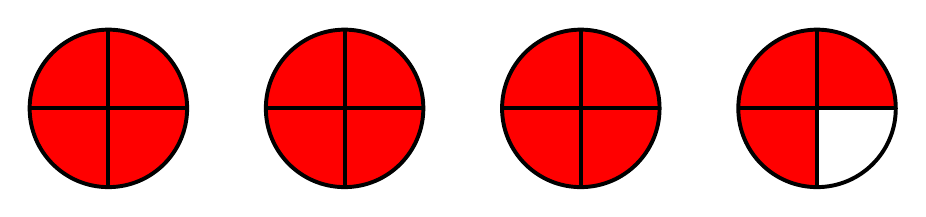
\begin{tikzpicture}
	\fill[red] (0,0) -- (0,1) arc (90:270:1cm) -- cycle;
	\fill[red] (0,0) -- (0,1) arc (90:-90:1cm) -- cycle;
	\draw[line width=0.5mm] (0,0) circle (1cm);
	\draw[line width=0.5mm] (-1,0) -- (1,0);
	\draw[line width=0.5mm] (0,1) -- (0,-1);
	
	\fill[red] (3,0) -- (3,1) arc (90:270:1cm) -- cycle;
	\fill[red] (3,0) -- (3,1) arc (90:-90:1cm) -- cycle;
	\draw[line width=0.5mm] (3,0) circle (1cm);
	\draw[line width=0.5mm] (-1+3,0) -- (1+3,0);
	\draw[line width=0.5mm] (0+3,1) -- (0+3,-1);
	
	\fill[red] (6,0) -- (6,1) arc (90:270:1cm) -- cycle;
	\fill[red] (6,0) -- (6,1) arc (90:-90:1cm) -- cycle;
	\draw[line width=0.5mm] (6,0) circle (1cm);
	\draw[line width=0.5mm] (-1+6,0) -- (1+6,0);
	\draw[line width=0.5mm] (0+6,1) -- (0+6,-1);
	
	\fill[red] (9,0) -- (9,1) arc (90:270:1cm) -- cycle;
	\fill[red] (9,0) -- (9,1) arc (90:0:1cm) -- cycle;
	\draw[line width=0.5mm] (9,0) circle (1cm);
	\draw[line width=0.5mm] (-1+9,0) -- (1+9,0);
	\draw[line width=0.5mm] (0+9,1) -- (0+9,-1);
	
\end{tikzpicture}
\captionof{figure}{A graph representing a mixed number}
\end{center}

In improper fraction format, the graph represents $\frac{15}{4}$, because there are $15$ pieces of a quarter.

In mixed number format, the graph represents $3\frac{3}{4}$.

This implies:
\[ \frac{15}{4} = 3\frac{3}{4}  \]

Let's look at both graphs and both conversions:
\[
\begin{aligned}[t]
	\frac{7}{3} &= 2\frac{1}{3} \\
	\frac{15}{4} &= 3\frac{3}{4}
\end{aligned}
\]

The fraction $\frac{7}{3}$ has two whole pies because $3$ goes into $7$ twice. The fraction part of $2\frac{1}{3}$ is $\frac{1}{3}$ because there is one extra piece, or $7\div3=2R1$ (remainder is $1$).

The fraction $\frac{15}{4}$ has three whole pies because $4$ goes into $15$ three times. The fraction part of $3\frac{3}{4}$ is $\frac{3}{4}$ because there are three extra pieces, or $15\div4=3R3$ (remainder is $3$).

Once the above explanation makes sense, we can convert between improper fractions and mixed numbers without graphing.

\begin{myexample}
Convert $\frac{19}{7}$ to a mixed number.
\end{myexample}
\begin{solution}
Since $19\div7=2R5$, it implies we can draw two whole pies, with each pie having $7$ pieces. There are still $5$ extra pieces, so we have:
\[ \frac{19}{7} = 2\frac{5}{7} \]
\end{solution}

\begin{myexample}
Convert $4\frac{3}{5}$ to a mixed number.
\end{myexample}
\begin{solution}
The mixed number's fraction part is $\frac{3}{5}$, implying each pie is cut into $5$ pieces.

Since there are $4$ whole pies, once each pie is cut into $5$ pieces, there are a total of $4\cdot5=20$ pieces.

The fraction part is $\frac{3}{5}$, implying there are $3$ extra pieces. Altogether, there are $4\cdot5+3=23$ pieces of one fifth of a pie. So we have: 
\[ 4\frac{3}{5} = \frac{4\cdot5+3}{5} = \frac{23}{5} \]
\end{solution}

\subsection{Mixed Numbers on Number Line}
The following figures show how to locate mixed numbers on the number line. These figures are pretty self-explanatory. We need to count each unit (like from 0 to 1) is cut into how many segments.

\begin{center}
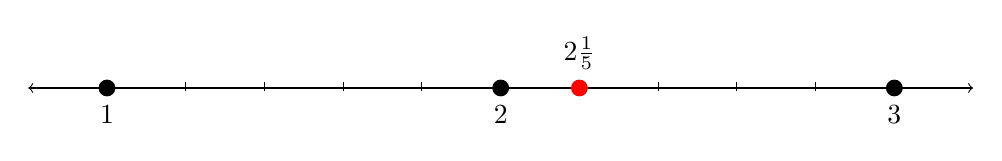
\begin{tikzpicture}
% a straight line segment
\draw [<->] (0,0) -- (12,0);
% the ticks and their labels
\foreach \x  in {1,...,11}
  \draw[xshift=\x cm] (0pt,2pt) -- (0pt,-1pt);
\node[fill=black,draw=black,circle,inner sep=2pt,label=below:{$2$}] at (6,0) {};
\node[fill=black,draw=black,circle,inner sep=2pt,label=below:{$3$}] at (11,0) {};
\node[fill=black,draw=black,circle,inner sep=2pt,label=below:{$1$}] at (1,0) {};
\node[fill=red,draw=red,circle,inner sep=2pt,label=above:{$2\frac{1}{5}$}] at (7,0) {};
\end{tikzpicture}

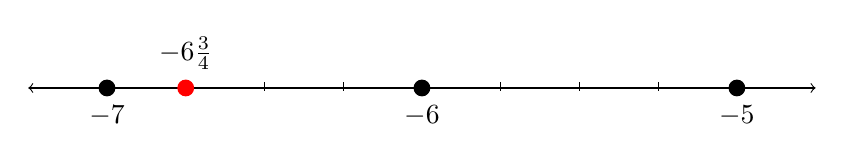
\begin{tikzpicture}
% a straight line segment
\draw [<->] (0,0) -- (10,0);
% the ticks and their labels
\foreach \x  in {1,...,9}
  \draw[xshift=\x cm] (0pt,2pt) -- (0pt,-1pt);
\node[fill=black,draw=black,circle,inner sep=2pt,label=below:{$-6$}] at (5,0) {};
\node[fill=black,draw=black,circle,inner sep=2pt,label=below:{$-5$}] at (9,0) {};
\node[fill=black,draw=black,circle,inner sep=2pt,label=below:{$-7$}] at (1,0) {};
\node[fill=red,draw=red,circle,inner sep=2pt,label=above:{$-6\frac{3}{4}$}] at (2,0) {};
\end{tikzpicture}

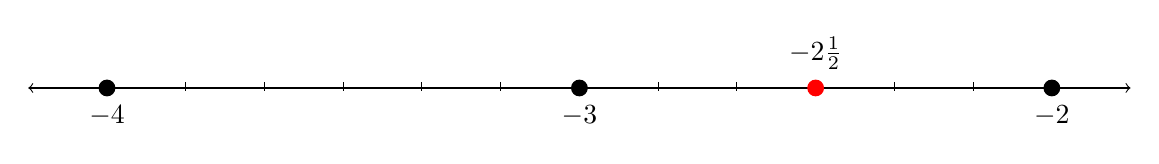
\begin{tikzpicture}
% a straight line segment
\draw [<->] (0,0) -- (14,0);
% the ticks and their labels
\foreach \x  in {1,...,13}
  \draw[xshift=\x cm] (0pt,2pt) -- (0pt,-1pt);
\node[fill=black,draw=black,circle,inner sep=2pt,label=below:{$-4$}] at (1,0) {};
\node[fill=black,draw=black,circle,inner sep=2pt,label=below:{$-3$}] at (7,0) {};
\node[fill=black,draw=black,circle,inner sep=2pt,label=below:{$-2$}] at (13,0) {};
\node[fill=red,draw=red,circle,inner sep=2pt,label=above:{$-2\frac{1}{2}$}] at (10,0) {};
\end{tikzpicture}
\captionof{figure}{Locate mixed numbers on number line}

\end{center}

On the last number line, note that the segment from $-4$ to $-3$ is cut evenly into $6$ pieces, implying each piece represents $\frac{1}{6}$.

The red dot represents $-2\frac{3}{6}$. We must reduce the fraction: $-2\frac{3}{6}=-2\frac{1}{2}$.

\subsection{Summary}
Let's review what we learned in this lesson:
\begin{itemize}
\item To change a mixed number to an improper fraction, we do:
\[ 3\frac{4}{5} = \frac{3\cdot5+4}{5} = \frac{19}{5} \]
\item To change an improper fraction to a mixed number, we first do a division:
\[ 19\div5=3R4 \]
Next we have:
\[ \frac{19}{5}=3\frac{4}{5} \]
Understand that the $3$ represents $3$ whole pies, and the $4$ represents $4$ extra pieces (the remainder).
\end{itemize}

